\label{chp:Experiments}
\section{Data set}
\label{sec:Dataset}
The Wi-Fi CSI signature dataset~\cite{moon2017air} at position 1 was used to test the proposed system. These dataset contained 10 signatures made by 98 people in each direction for a total of 980 signatures made in each direction, as shown in~\ref{tab_dataset}. The size of each sample had a data resolution of 500 x 30 x 6. 
\textbf{
Visualization of CSI signature data is shown in Fig.~\ref{fig_csi}.}
%fig:csi
\begin{figure}[!ht]
    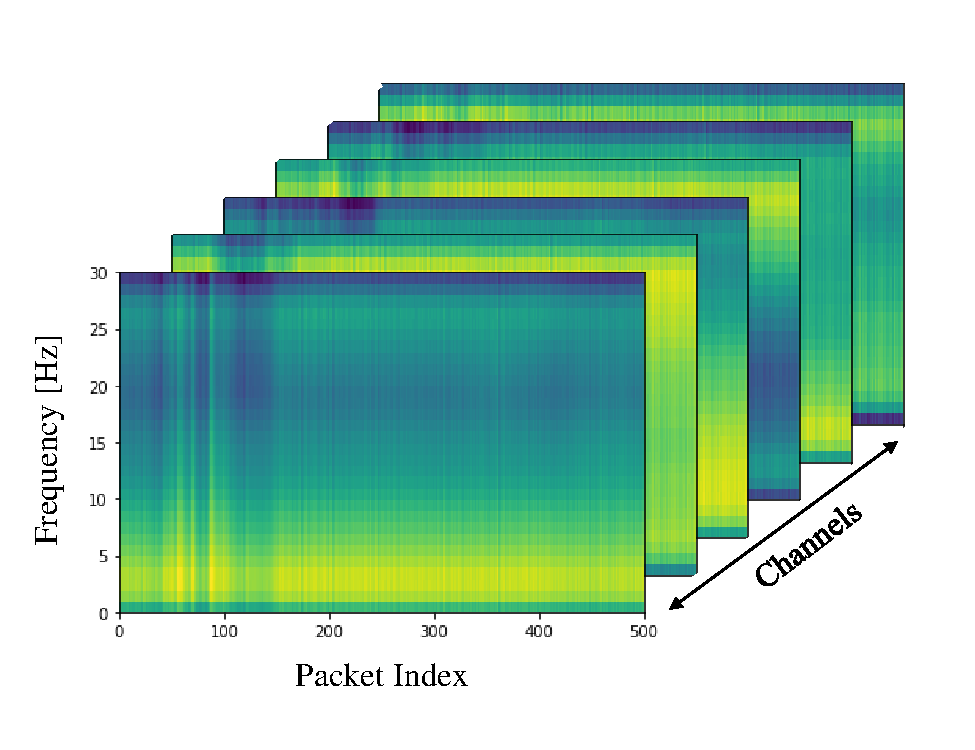
\includegraphics[width=\textwidth]{fig_csi_v2.pdf}
    \caption{Visualization of CSI signal. This data consists of signal strengths for 30 subcarriets per 500 time packet with 6 channels. Each subcarrier corresponds to the frequency, and the intensity value indicates the signal strength.} \label{fig_csi}
\end{figure}
%tab:dataset
\begin{table}
    \caption{Description of the Dataset.}
    \label{tab_dataset}
    \begin{tabular}{ccc}
    \hline
    Direction of signature & \# of identities & \# of data \\ 
    \hline
    1                      & 98               & 980        \\ 
    2                      & 98               & 980        \\ 
    3                      & 98               & 980        \\ 
    4                      & 98               & 980        \\ 
    \hline
    \end{tabular}
\end{table}

\section{Experimental Parameters}
%performance
To compare the proposed method's feature extraction performance to that of traditional and deep-learning based methods, feature space was visualized as a 2D Euclidean plane using principal component analysis (``PCA''). 
% handcraft
The proposed method's and traditional methods and deep-learning based methods.
For handcraft methods' least square estimations (``LSE'')~\cite{duda2012pattern}, PCA with LSE~\cite{turk1991eigenfaces}, support vector machine~\cite{vapnik2013nature} and the total error minimization with reduced multivariate polynomials~\cite{toh2003fingerprint,toh2008between} were compared. Parameters were selected that performed optimally in each traditional method. For LSE,SVM, and TER, the input signatures were reduced to 500$\times$30 by averaging the subcarrier axis. For PCA-LSE, the input signature dimension was reduced to 40 following~\cite{moon2017air}. For SVM with a Gaussian kernel function (``RBF''), the kernel's parameters $c$ and $\gamma$ were chosen by a grid search over the range $c\in\{0.01,1,10\}$ and $\gamma\in\{0.01/3000, 0.1/3000, 1/3000, 10/3000, 100/3000\}$. For TER, the parameter M was chosen from among $M\in\{1,2,3\}$ and $\tau=\eta=0.5$ following~\cite{toh2008between}.
For comparison with deep-learning based methods, Siamese network~\cite{koch2015siamese} and baseline triplet network~\cite{hoffer2015deep} were used.
The proposed method was compared to Siamese networks~\cite{koch2015siamese} and baseline triplet networks~\cite{hoffer2015deep} as deep learning based methods.
%protocols
Verification performance was evaluated in terms of the equal error rate (``EER''). Random five-runs of two-fold cross-validation tests were conducted.
Due to hardware memory limitations, the number of negative pairs used was reduced to the number of positive data pairs used for calculating the EER for a total of 18,620 pairs.
% KAR structure
The structure of the KAR learning MLP sub-networks in the proposed system is shown in~\ref{kar_structure}. The three layers' sizes were set to 1,024, 64 and 16. The size of the third layer was equal to the number of feature vectors of the proposed ConvNet. The weights in the layers were initialized in a normal distribution between 0 and 1 before training.
$tan^{-1}$ was used as an active function following~\cite{toh2018analytic}.
\begin{table}[]
    \caption{KAR space learning network structure.}
    \label{kar_structure}
    \centering
    \begin{tabular}{|l|l|l|}
    \hline
    Layer   & Size     & Activation Function \\ \hline
    Input   & 500$\times$30$\times$6 &            \\
    Fully-connected 1 & 1$\times$1$\times$1024 & $\sigma = {tan}^{-1}$     \\
    Fully-connected 2 & 1$\times$1$\times$64 & $\sigma = {tan}^{-1}$     \\
    Fully-connected 3 & 1$\times$1$\times$16  & $\sigma = {tan}^{-1}$     \\
    Output  & 1$\times$1$\times$50   &            \\ \hline
    \end{tabular}
\end{table}
% conv structure
The same ConvNet structure shown in~\ref{conv_structure} and parameters were used for the proposed and deep learning based methods. The CovNet structure consisted of three 3$\times$3 convolution filters and stride one. A ReLU activation function and 2$\times$2 max-pooling layers were applied between the filters. The depth of each layer was set to \{64,128,256\}. The output layer with sigmoid activation was regularized according to $L2$ with a penalty of 0.0001. The size of the final feature vectors was 16.
\begin{table}[]
    \caption{ConvNet model structuer.}
    \label{conv_structure}
    \centering
    \begin{tabular}{|c|c|c|c|}
    \hline
    Layer     & Activation Function & Kernel / Stride & Input Size \\ \hline
    Conv 1    & ReLU       & (3$\times$3)$\times$64/1      & 500$\times$30$\times$6   \\
    MaxPool 1 &            & (2$\times$2)/1         & 500$\times$30$\times$64  \\
    Conv 2    & ReLU       & (3$\times$3)$\times$128/1     & 250$\times$15$\times$64 \\
    MaxPool 2 &            & (2$\times$2)/1         & 250$\times$15$\times$128 \\
    Conv 3    & ReLU       & (3$\times$3)$\times$256/1     & 125$\times$8$\times$128  \\
    MaxPool 3 &            & (2$\times$2)/1         & 125$\times$8$\times$256  \\
    Fully-connected     & Sigmoid    & 16             & 63$\times$4$\times$256   \\
    L-2 Norm  &            &                 & 1$\times$1$\times$16    \\
    Concat    &            &                 & 1$\times$1$\times$16    \\ \hline
    \end{tabular}
\end{table}
% traning parameters
The deep learing network was trained with a learning rate of 0.0005, 3,000 iteration, and a mini-batch size of 32. The Adam optimizer was used to calculate the loss function. The ConvNet structures were initialized before training following~\cite{koch2015siamese}. The convolution filters used a normal distribution with a mean of 0 and a standard deviation of 0.0001. The biases used normal distribution with a mean of 0.5 and a standard deviation of 0.01. Triplet loss was calculated with an alpha value of 0.5.

%5.3. Experimental results
\section{Experimental Results}
%5.3.1. verification performance
\subsection{Performance}
\ref{tab_performance} shows the average EER from the first experiment generated by five-runs of two-fold cross-validation tests under optimal parameter settings. The proposed method had an EER of 19.35\%, out-performing both the traditional and deep learning based methods (Table~\ref{tab_performance}).
Deep learning based methods out-performed the traditional methods because they utilized the entire input signal and had better feature extraction abilities.
\begin{table}[!h]
    \caption{Average EER of five-runs of two-fold cross-validation tests.}\label{tab_performance}
    \centering
    \begin{tabular}{|c|c|c|}
    \hline
    Methodology   &   Best EER (\%) &   Condition   \\  \hline
    LSE &   48.44   &  - \\ 
    PCA-LSE    &   30.79   &  Reduced dimension=40    \\
    SVM (Linear) &   28.23   &   c=1 \\
    SVM (RBF)    &   24.31   &   c=1, $\gamma$=0.01/3000 \\
    TER-RM2 &   35.84   &  M=1,$\tau$=$\eta$=0.5   \\     \hline
    Siamese network  &   23.53   &   lr=0.00005  \\
    Baseline triplet network &   20.34   &   lr=0.00005, $\alpha$=0.1  \\
    \textbf{Proposed system} &   \textbf{16.67}   &  \textbf{lr=0.00005, $\alpha$=0.1}  \\
     \hline
    \end{tabular}
\end{table}

%roc
The proposed method had the widest area under the receiver operating characteristic (``ROC'') curve (Fig.~\ref{fig_roc}).
\begin{figure*}[!ht]
    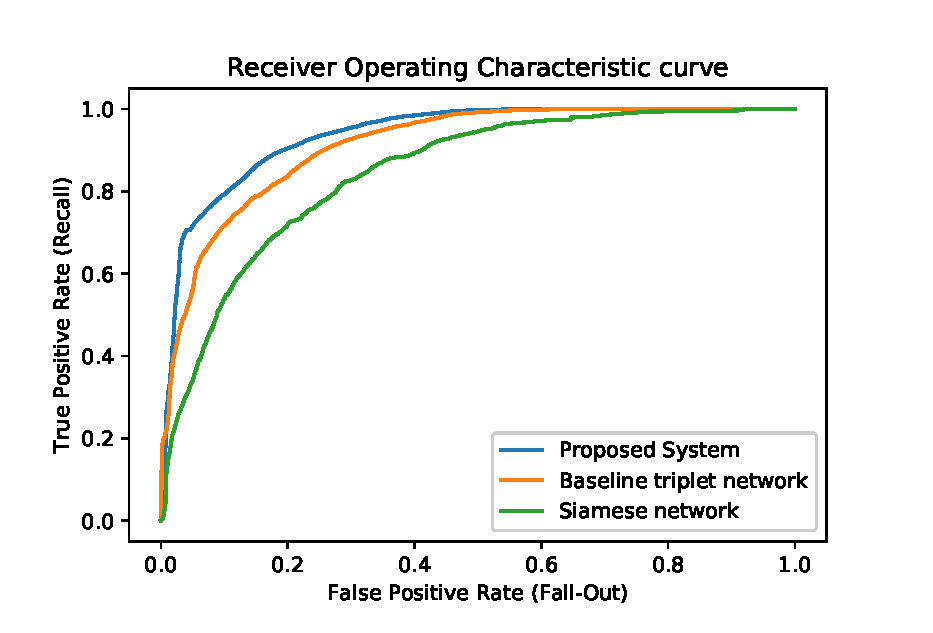
\includegraphics[width=\textwidth]{fig_roc_v15.eps}
    \caption{Normalized training loss curve.} \label{fig_roc}
\end{figure*}
 %5.3.1. conv speed
\subsection{Convergence Speed}
Fig.~\ref{fig_loss} shows the convergence of the normalized loss function during training. The proposed method had a faster convergence speed than the deep learning based methods, indicating that KAR learning accelerated the learning speed.
 \begin{figure*}[!ht]
    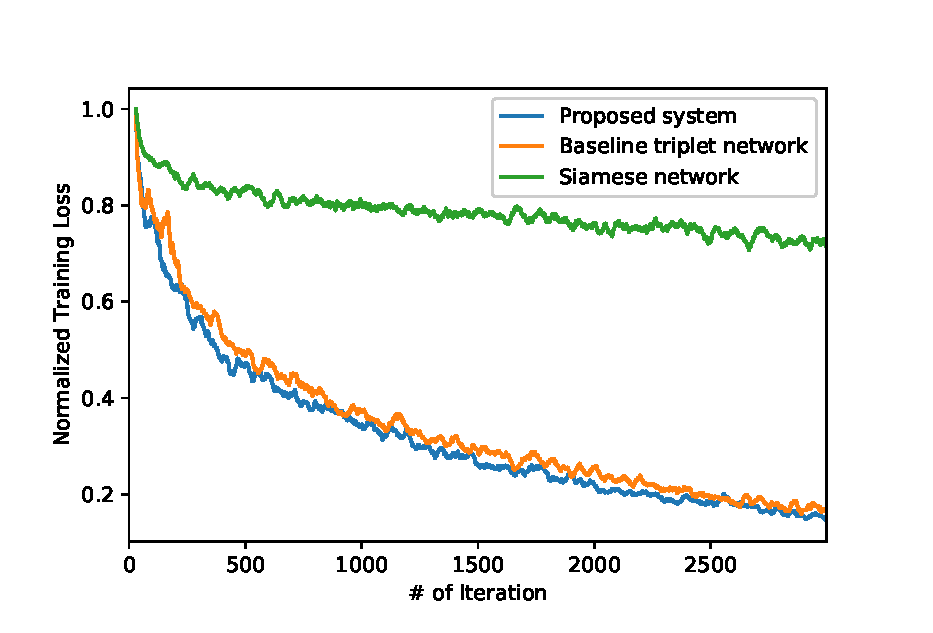
\includegraphics[width=\textwidth]{normalized_loss_curve_ma30_v3.eps}
    \caption{normalized training loss trends} \label{fig_loss}
\end{figure*}
%5.3.2. feature vector
\subsection{Feature Vector Size Effect}
Fig.~\ref{fclayer} shows the EERs for different sizes of feature vectors in the feature space. 
For metric learning systems, feature vector size is generally positively correlated with system performance.
The proposed system's performance was negatively correlated with feature vector size.
\begin{table}[]
    \centering
    \begin{tabular}{|l|l|l|l|l|}
    \hline
    Feature vector size        & 16    & 8     & 4     & 2     \\ \hline
    Siamese network            & 20.34 & 22.05 & 29.39 & 34.26 \\ \hline
    Baseline triplet network   & 18.37 & 19.52 & 19.20 & 24.76 \\ \hline
    Proposed method            & 16.67 & 18.03 & 18.08 & 26.64 \\ \hline
    \end{tabular}
\end{table}
\begin{figure}[!ht]
    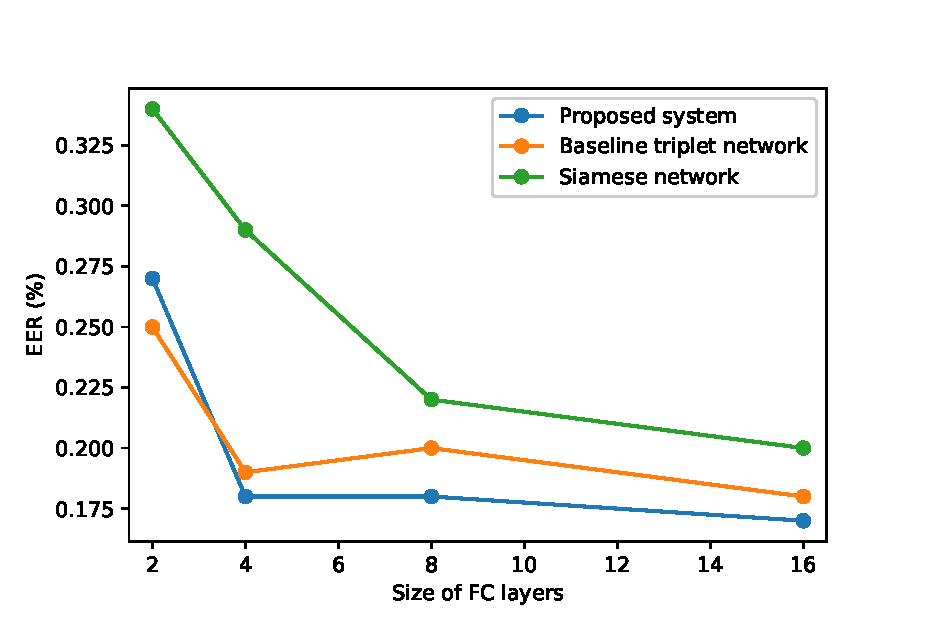
\includegraphics[width=\textwidth]{fclayer_v1.eps}
    \caption{Feature Vector Size Effect.} \label{fclayer}
\end{figure}
\iffalse
% Omitted: 5.3.3. 2D visualization of feature vector
\subsection{2D Visualization of the Feature Vectors}
\begin{figure}[!ht]
    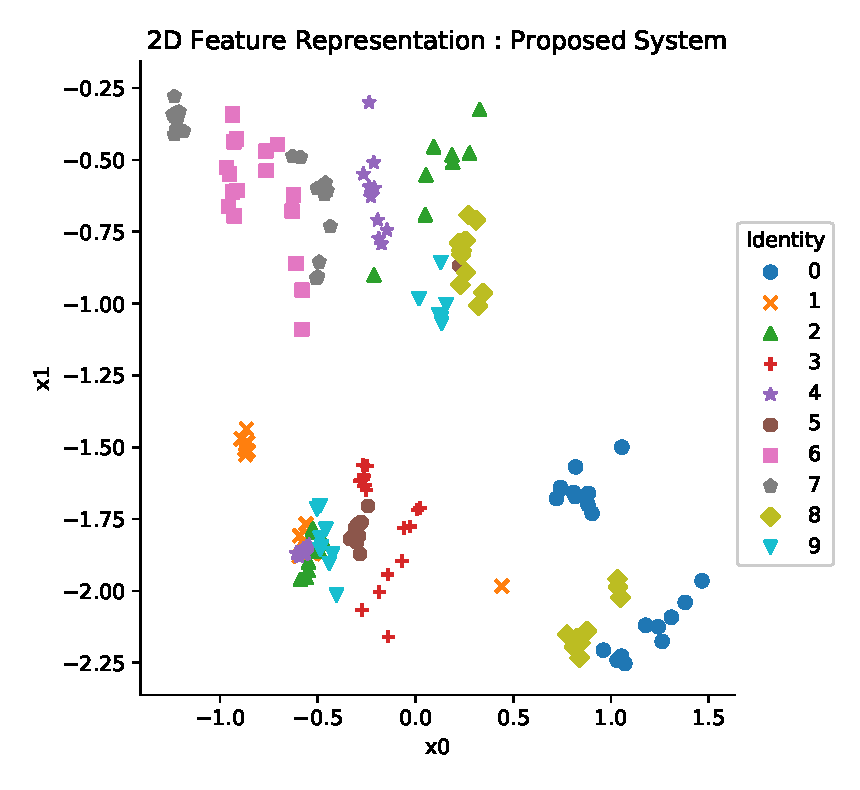
\includegraphics[width=\textwidth]{fig_2d_triKAR_10_v1.eps}
    \caption{2D Feature Representation : Proposed System.} \label{fig_2d_triKAR_10}
\end{figure}
\begin{figure}[!ht]
    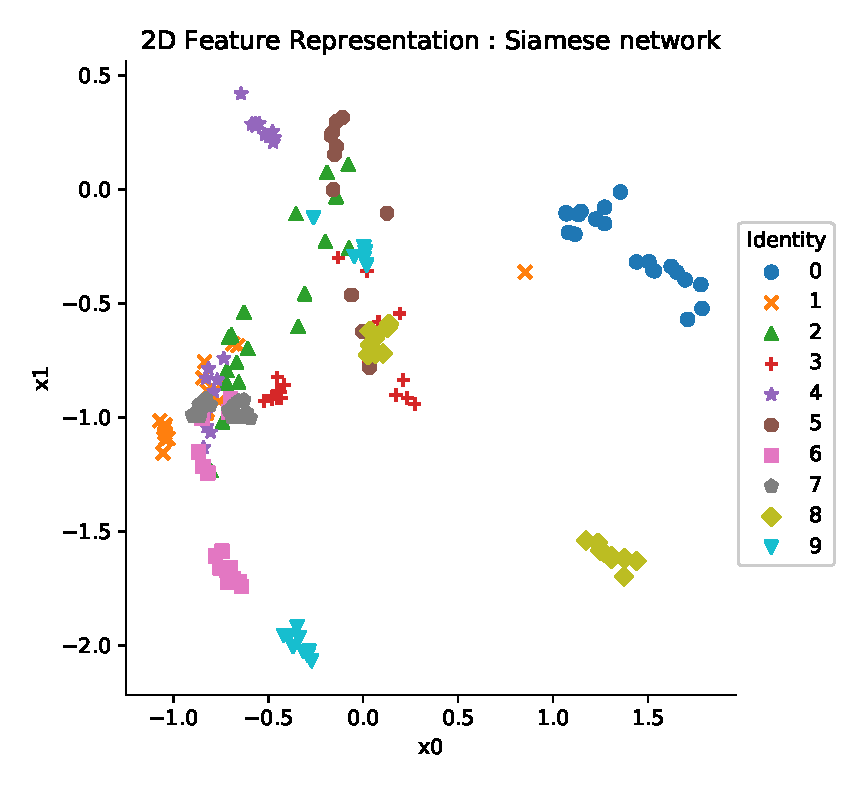
\includegraphics[width=\textwidth]{fig_2d_tribase_10_v1.eps}
    \caption{2D Feature Representation : Baseline triplet network.} \label{fig_2d_tribase_10}
\end{figure}
\begin{figure}[!ht]
    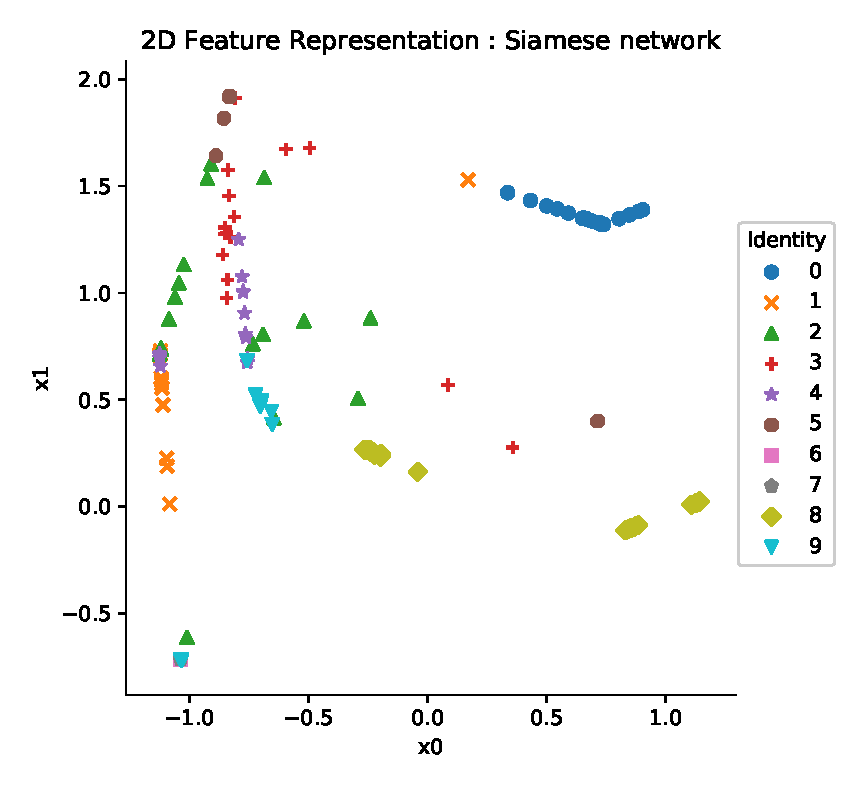
\includegraphics[width=\textwidth]{fig_2d_siam_10_v1.eps}
    \caption{2D Feature Representation : Siamese network.} \label{fig_2d_siam_10}
\end{figure}
To visualize the proposed system's feature extraction performance, the feature space was projecgted onto two-dimensional Euclidean space using PCA (Figs.~\ref{fig_2d_siam_10},~\ref{fig_2d_triKAR_10}, and~\ref{fig_2d_tribase_10}). each system's feature extraction performance by determining whether proximate points shared the same identity. Only the first 10 identities were visualized to facilitate the visual confirmation process.
The proposed method used the space most efficiently. The Siamese network linearly arranged feature vectors, making it difficult to distinguish between classes. The baseline triplet network caused many identities to overlap.
\fi
%5.3.3. Comparision between mining methods
\subsection{Comaprison between mining algorithms}
\textbf{
In this section, the proposed system is compared to a triplet network that adopted different mining methods. The methods used for mining are the traditional methods given in Table \ref{tab_dataset}. 
We also compared Extreme Learning Machine (``ELM'').
ELM is a fast-learning SLFN network which uses an analistic method for calculating the weight of the network~\cite{huang2006extreme}.
For the traditional methods, the input signals are resized to 500 × 30 by averaging along the subcarrier axes due to limitation of hardware memory.}

\textbf{
Table \ref{tab_mining} shows the test EER of proposed and compared triplet mining methods. 
TER-RM2 showed the best test EER performance in this case. Proposed system (KAR learning) showed slightly worse performance of 16.67\% EER. SVM also showed good performance.
From this result, it can be seen that the traditional method can increase the accuracy of the triplet network when applied to the triplet mining.
}

\begin{table}[!h]
    \caption{Average EER between mining methods.}\label{tab_mining}
    \centering
    \begin{tabular}{|c|c|c|}
    \hline
    Methodology   &   Best EER (\%) &   Condition   \\  \hline
    LSE &   19.03   &  - \\ 
    SVM (Linear) &   17.48   &   c=1 \\
    SVM (RBF)    &   17.31   &   c=1, $\gamma$=0.01/3000 \\
    ELM &   17.02   &   layer=[1024,16] \\
    TER-RM2 &   16.37   &  M=1,$\tau$=$\eta$=0.5   \\     \hline
    \textbf{Proposed System} &   \textbf{16.67}   &  \textbf{layer=[1024,64,16]}  \\
     \hline
    \end{tabular}
\end{table}